%%%%%%%%%%%%%%%%%%%%%%%%%%%%%%%%%%%%%%%%%
% Beamer Presentation
% LaTeX Template

\documentclass{beamer}
\mode<presentation> {
% Theme
\usetheme{metropolis}
%\usetheme[background=dark]{metropolis}
%\setbeamertemplate{footline} % To remove the footer line in all slides uncomment this line
%\setbeamertemplate{footline}[page number] % To replace the footer line in all slides with a simple slide count uncomment this line
%\setbeamertemplate{navigation symbols}{} % To remove the navigation symbols from the bottom of all slides uncomment this line
}

%Packages
\usepackage{graphicx} % Allows including images
\usepackage{booktabs} % Allows the use of \toprule, \midrule and \bottomrule in tables
%\usepackage{cite}
\usepackage[numbers]{natbib} % For bibliography
\usepackage{multirow}
\usepackage{hyperref}
%\usetheme{Warsaw}
\usepackage[absolute,overlay]{textpos}


% Prepare title and TOC
\title[Short title]{Reproducible Research -- practical} 
\author{Marco Chiapello} 
\institute[Center for Proteomics] 
{
Center for Proteomics\\
University of Cambridge \\ 
\medskip
\textit{mc983@cam.ac.uk} 
}
\date{\today} 

%\AtBeginSection[]
%{
%\begin{frame}<beamer>
%\frametitle{Overview}
%\tableofcontents[currentsection]
%\end{frame}
%}


%-------------------------------------------
% MAIN DOCUMENT
%-------------------------------------------
\begin{document}

%-------------------------------------------
% TITLE PAGE
%-------------------------------------------
\begin{frame}
\titlepage 
\end{frame}

%----------------------------------------------------------------------------------------
%	PRESENTATION SLIDES
%----------------------------------------------------------------------------------------

%-----------
% Exercise 1 
%-----------
\begin{frame}
    \frametitle{Exercise 1}
    {\sc GOAL: create a default minimal document}
    \begin{itemize}
        \item Open RStudio
        \item Select File $>$ New file $>$ R Markdown
        \item Create an HTML document
    \end{itemize}
\end{frame}
%-----------------------
\begin{frame}
    \frametitle{Exercise 1}
    \begin{center}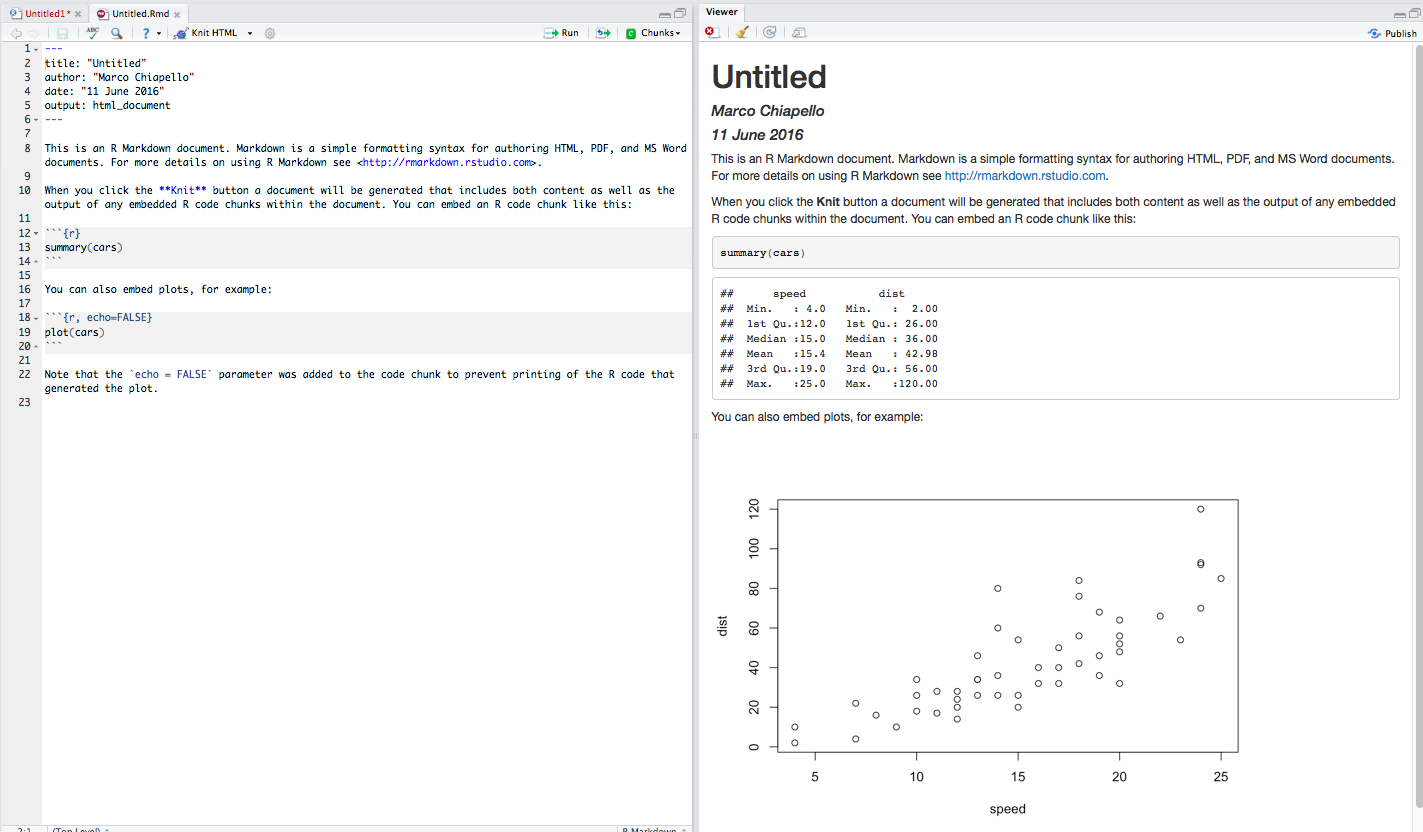
\includegraphics[scale=0.23]{figures/RmarkdownExample.png}\end{center}
\end{frame}



\end{document}
